\section{The Decomposition: Perception, Recognition, Knowledge, and Intelligence}


\subsection{Overview}


\S{}1.2 で本論文の問題提起 ── 知性は停止構造ではなく、停止構造を生み出し続ける運動である ── を提示した。本セクションはこの主張を構造的に支える層分離を行う。具体的には、知性論において頻繁に混同される四つの概念 ── \textbf{知覚(perception)}、\textbf{認識(recognition)}、\textbf{知識(knowledge)}、\textbf{知性(intelligence)} ── を、互いに異なる構造層に属するものとして分離する。

本セクションの目的は古典的定義の精緻化ではない。各概念がそもそも \textbf{異なる種類の構造的対象} を指していることを示し、これらを同一平面で論じる限り知性論が破綻し続けることを構造的に示すことである。

この分離は本論文全体の中心主張であり、\S{}3 の公理系、\S{}6 の Gettier 問題再定位、\S{}7 の正しさの不安定化、\S{}8 の個体内非閉論証 ── これらすべては本セクションで提示する層分離を前提として初めて成立する。

\subsection{The structural distinction: stopping versus ongoing}


四概念に立ち入る前に、本セクションを貫く一つの構造的区別を明示する。それは \textbf{停止構造(stopping structure)} と \textbf{持続運動(ongoing dynamics)} の区別である。

\textbf{停止構造} とは、ある時点で状態が固定され、後の参照・伝達・操作の対象となる構造である。停止構造は静的に保持され、それ自体は動かない。書物の頁、データベースのレコード、信号の凍結像、命題の真偽値 ── これらはすべて停止構造の例である。停止構造の特徴は \textbf{保存可能性(storability)} にある。

\textbf{持続運動} とは、それ自身の動力学によって変形を続ける構造である。持続運動は停止構造を内部に生み出すこともあるが、運動自体は保存対象ではない。流れる川の水流、走り続ける反応系、改訂を続ける推論過程 ── これらは持続運動の例である。持続運動の特徴は \textbf{再改訂可能性(revisability)} にある。

この二つは互いに転換不可能である。停止構造は持続運動を生まないし、持続運動は停止構造に格納されない。両者を混同すること ── すなわち停止構造に持続運動の性質を担保させようとすること、あるいは持続運動を停止構造の集合として記述しようとすること ── が、本論文が後続セクションで指摘する知性論の構造的失敗の源泉である。

四概念は、この区別に対して以下のように整列する:

\begin{itemize}
\item \textbf{知覚} と \textbf{認識} は、停止構造でも持続運動でもなく、両者の間にある \textbf{前駆層}(状態形成)である
\item \textbf{知識} は典型的な停止構造である
\item \textbf{知性} は典型的な持続運動である
\end{itemize}

以下、各概念を順に検討する。

\subsection{Perception as input-state formation}


\textbf{知覚} を、入力信号から内部状態が形成される事象として扱う。

ここで「内部状態」とは認識主体の状態空間における何らかの可区別な点を指し、その時点での \textbf{意味}・\textbf{正しさ}・\textbf{真偽} は問われない。何らかの信号がシステム内で \textbf{利用可能(available)} になった ── ただそれだけが知覚の条件である。

この扱いは Gibson (1986) の生態学的知覚論と部分的に重なる \citep{Gibson1986}。Gibson は知覚を「環境からの affordance の検出」として扱い、信号の真偽判定や表象化を知覚の前提条件としなかった。本論文の知覚概念も同様に、表象化や正当化の手前の事象として知覚を位置づける。

ただし本論文では Gibson の生態学的詳細には立ち入らない。本論文にとって重要なのは、\textbf{知覚は停止構造ではなく、停止構造の素材を提供する事象である} という点のみである。知覚はそれ自体としては不安定で、即座に減衰しうるか、後続の処理によって安定化されるかのいずれかとなる。

知覚の構造的役割は以下に要約される:

\begin{quote}
知覚は、信号が後続の動的処理に \textbf{接続可能な状態} となる事象である。
知覚はまだ知識ではなく、まだ知性でもない。
\end{quote}

\subsection{Recognition as mapping into an existing representational structure}


知覚状態はそれ自体としては典型的に不安定である。多くの系は、知覚を既存の表象構造に \textbf{写像} することで、後続の動的処理に渡せる形に変換する。この写像を \textbf{認識(recognition)} と呼ぶ。

認識は知覚と知識の \textbf{中間層} である。それは:

\begin{itemize}
\item 知覚以上のものである ── 単なる状態形成ではなく、既存構造への割当が行われている
\item 知識未満のものである ── まだ停止しておらず、log として保存されているわけでもない
\item 知性そのものではない ── それ自体は動的な改訂を行わず、既成のスキーマに従って機械的に行われる
\end{itemize}

認識を独立層として立てることには明確な理由がある。哲学的議論では「知覚」と「知識」のあいだに往々にして大きな間隙があり、その間隙を埋めるために「正当化」「証拠」「信念形成」などの曖昧な概念が持ち込まれてきた。本論文の枠組みでは、この間隙は構造的に明確な層 ── すなわち認識 ── によって埋められる。

ただし重要な但し書きとして、認識が依拠する「既存の表象構造」自体は、過去の知性的動態の \textbf{沈殿物} として形成されたものである。認識は機械的だが、その基盤は知性の歴史を持つ。この点が \S{}2.6 で扱う層間結合の鍵となる。

\subsection{Knowledge as stabilized stopping (log)}


\textbf{知識} を、安定化された停止構造として扱う。

この扱いにおいて、知識の定義的特徴は \textbf{正しさではなく安定性} である。知識は log のような対象であり、保存・参照・伝達が可能である。それは正しいか誤っているか、正当化されているか否か ── これらの属性は知識が \textbf{持ちうる} 属性ではあるが、知識を知識たらしめる \textbf{本質的属性} ではない。

知識の本質的属性は、それが \textbf{動かない} 点にある。知識は再利用可能な停止点として、後続の処理から繰り返し参照されうる。この再利用可能性こそが知識の機能であり、同時にその構造的限界でもある。

この扱いは古典的な「真であり、信じられており、正当化された命題(JTB)」とは異なる。JTB 定義は知識を \textbf{真理保持の停止構造} として扱い、Gettier (1963) 以来の半世紀以上にわたる反例の連鎖を生んだ。本論文の知識概念は、真理保持ではなく \textbf{安定化された参照可能性} に本質を置く。

知識が動かないという点は、結果として重要な帰結を持つ:

\begin{quote}
知識が改訂されるとき、改訂を行うのは知識自身ではない。
改訂は、知識の \textbf{外側にある動力学}(すなわち知性)によって遂行される。
\end{quote}

この点は \S{}7 で正しさの累積が知性を安定化させない理由として、また \S{}8 で個体内非閉論証の前提として、繰り返し参照される。

\subsection{Intelligence as ongoing, revisable dynamics}


\textbf{知性} を、知覚・認識・知識を \textbf{運用しながら、自身は停止しない} 持続運動として扱う。

知性は知覚でも認識でも知識でもない。知性とは、これら三者を素材として動き続け、新たな停止構造(認識スキーマの更新、知識の追加・修正)を生み出しながら、同時にその停止構造を \textbf{改訂可能な状態に保ち続ける} 運動である。

知性の本質的属性は、\textbf{持続性(persistence)} と \textbf{再改訂可能性(revisability)} の同時保持にある。知性は停止しない ── これは知性が答えを持たないという意味ではなく、いかなる答えも常に再改訂の対象として保持され続けるという意味である。

この扱いから直ちに以下が帰結する:

\begin{quote}
知性はオブジェクトとして完全に格納されることがない。
格納されうるのは、知性の停止生成物(logs)のみである。
知性そのものは、それらを生み出し、改訂し続ける \textbf{動き} である。
\end{quote}

これは単なる定義上の主張ではない。これは \S{}3 で公理化される三条件(連結状態空間・時間順序・グローバル制約 $\Phi$)の \textbf{同時必要性} が示す構造的事実である。停止構造としての知性は、これら三条件のうち少なくとも一つを欠く ── ゆえに知性は停止構造として記述できない。

\subsection{Why conflation occurs: the operational coupling of layers}


四層が互いに異なる構造に属するとしても、運用上は密接に結合している。この \textbf{運用上の結合} が、層分離を見えにくくし、混同を生む原因である。

具体的には:

\begin{itemize}
\item 知性的動態は、しばしば \textbf{より多くの知識を生成する}。これは知性の副産物だが、両者の区別を見えにくくする
\item 知性的動態は、しばしば \textbf{認識スキーマを更新する}。これも知性の副産物だが、認識と知性の境界を曖昧にする
\item 知識の蓄積は、しばしば \textbf{知性的動態の効率を高める}。これは事実だが、知識自体が知性を構成するわけではない
\item 認識の精緻化は、しばしば \textbf{知覚の粒度を変化させる}。これも事実だが、認識が知覚を生むわけではない
\end{itemize}

これらの結合関係は実在するが、いずれも \textbf{副産物} または \textbf{道具的支援} であって、層の同一性を意味しない。

これを比喩的に述べれば次のようになる:川は河岸を作り、河岸は川の流路を制約する ── だが川は河岸ではなく、河岸は川ではない。知性は知識を生み、知識は知性の運用を支える ── だが知性は知識ではなく、知識は知性ではない。

この比喩は \S{}10 で再び現れる。本論文が定式化する制約のうちのいくつかは、まさに「持続運動が停止構造の蓄積によっては安定化しない」という構造的事実を扱う(\S{}7)。

\subsection{Summary of the decomposition}


本セクションの層分離を以下に要約する。

\begin{table}[H]
\centering
\small
\begin{tabularx}{\textwidth}{>{\raggedright\arraybackslash}X>{\raggedright\arraybackslash}X>{\raggedright\arraybackslash}X>{\raggedright\arraybackslash}X}
\toprule
層 & 構造的種類 & 本質的属性 & 例 \\
\midrule
\textbf{知覚} & 前駆層 & 利用可能性(availability) & 信号が状態となる \\
\textbf{認識} & 前駆層 & 写像可能性(mappability) & 状態が既存スキーマに割り当てられる \\
\textbf{知識} & 停止構造 & 安定性(stability) & 命題、log、データベース \\
\textbf{知性} & 持続運動 & 再改訂可能性(revisability) & 推論過程、適応的動態 \\
\bottomrule
\end{tabularx}
\end{table}


この分離は本論文全体の構造的前提である:

\begin{itemize}
\item \S{}3 では、知性層に対応する持続運動の最小公理(三条件)を提示する
\item \S{}6 では、Gettier 問題が \textbf{知識層と知性層の混同に起因する診断装置} として再定位される
\item \S{}7 では、知識(停止構造)の累積が知性(持続運動)を \textbf{逆に不安定化させる} 動力学的帰結が示される
\item \S{}8 では、個体内において持続運動を停止させる演算子が \textbf{存在しえない} ことが論証される
\item \S{}9 では、これらすべての帰結が要請する越境境界 ── \emph{the differential horizon of intelligence} ── に名前が与えられる
\end{itemize}

本セクションの中心的主張は、最小限のかたちで次のように述べられる:

\begin{quote}
知性とは、停止構造ではなく、停止構造を生み出し続けながら、
自身は決して停止しない持続運動である。
この層分離なしには、知性のいかなる構造的理解も成立しない。
\end{quote}

\begin{figure}[H]
\centering
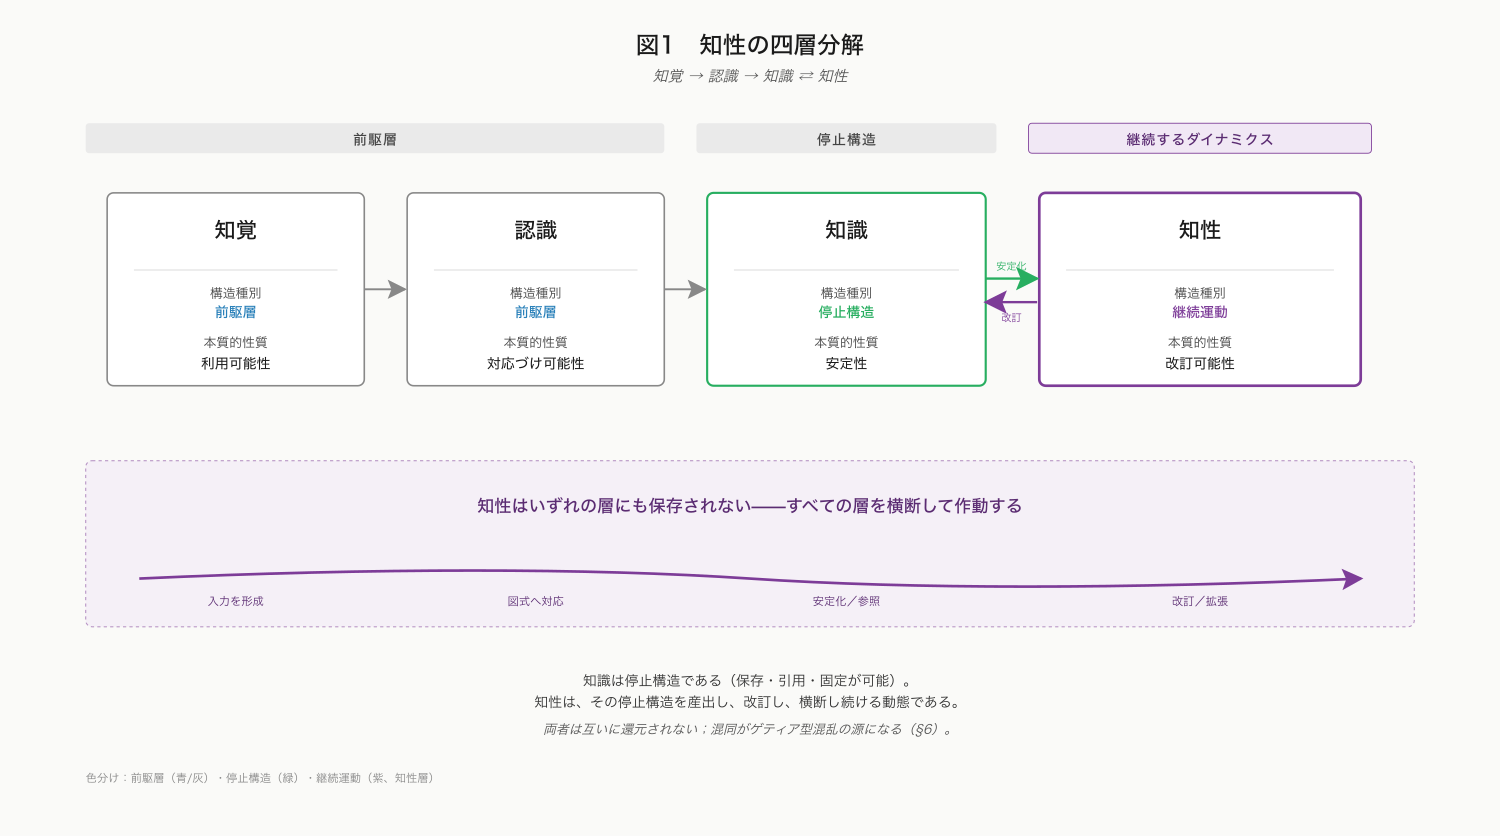
\includegraphics[width=\textwidth]{figures/fig1_four_layer_decomposition_ja.png}
\caption{四層分離の構造図(知覚 → 認識 → 知識 ⇄ 知性、知性は四層全体を運用するが、知性自身は格納されない)}
\label{fig:intelligence_part1_1}
\end{figure}
